% \renewcommand{\thechapter}{\Roman{chapter}}
\chapter{Characteristics of Malayalam Orthography}
\label{app:app1}

% %%%%%%%%%%%%%%%%%%%%%%% CHAPTER - 3 %%%%%%%%%%%%%%%%%%%%\\
% \chapter{Nature of Malayalam Orthography}
% \label{ch:NatureofOrthography} %%%%%%%%%%%%%%%%%%%%%%%%%%%%
\graphicspath{{Figures/appendix1/}}





% \section{Introduction}

Malayalam is a language spoken predominantly in the state of Kerala in southern India, with about 38 million native speakers. It belongs to the Dravidian language family, and has an alphasyllabary writing system \cite{bri1999typology}. Though Malayalam script is largely phonemic in nature, there are some unique characteristics like: (i) consonants with and without inherent vowel, (ii) consonant clusters with pronunciation different from the consonants present in them, (iii) special symbol \textit{virama}, that contextually chooses its function depending on its position in a word and (iv) graphemes being overloaded with non-native sounds in loan words. %\footnote{See Section \ref{arch} for details}. 



\begin{sidewaystable}[htpb]

  
			\caption{Short and long vowels in Malayalam and their IPA representations}\label{vowelgrapheme}%
			\begin{tabular}{@{}l|llllllllllllllll@{}}
				\hline \hline
		Vowels   & {\mal അ} {\ipa a}& {\mal ആ} {\ipa aː}   & {\mal ഇ} \ipa{i} & {\mal ഈ} \ipa{iː }  & {\mal ഉ} {\ipa u} & {\mal ഊ} {\ipa uː}  & {\mal ഋ} {\ipa rɨ} & {\mal ൠ} {\ipa rɨː}& {\mal ഌ} {\ipa lɨ} & {\mal ൡ} {\ipa lɨː}& {\mal എ} {\ipa e} & {\mal ഏ} {\ipa eː }& {\mal ഐ} {\ipa ai}      & {\mal ഒ} {\ipa o} & {\mal ഓ} {\ipa oː} & {\mal ഔ} {\ipa au}\\ \hline
             
				Vowel Signs  & {\mal }           & {\mal ാ}           & {\mal ി}         & {\mal ീ}           & {\mal ു}           & {\mal ൂ} & {\mal ൃ}            & {\mal ൄ}             & {\mal ൢ}            & {\mal ൣ}            & {\mal െ}          & {\mal േ}     & {\mal ൈ}                & {\mal ൊ}          & {\mal ോ}         & {\mal ൗ ൌ}     \\
				\hline
			\end{tabular}


\vspace{2cm}
 

 \begin{threeparttable}
  \caption{Consonants in Malayalam and their IPA representations}\label{consonantgrapheme}
			% \setcounter{mpfootnote}{\value{footnote}}
			% Redefine the command that produces the footnote number
			% \renewcommand{\thempfootnote}{\arabic{mpfootnote}}
			\begin{tabular*}{\textwidth}{@{\extracolsep{\fill}}llccccccccccc@{\extracolsep{\fill}}}
				\hline% \hline
				\textbf{Place of }& \multicolumn{9}{@{}c@{}}{\textbf{Manner of Articulation}}\\
				\textbf{Articulation} & Plosive\tnote{a} & Plosive\tnote{b} & Plosive\tnote{c} & Plosive\tnote{d}                        & Nasal        & Trill        & Tap          & Fricative   & Approximant      & Lateral                                               \\

				\hline
				Velar                        & {\mal ക} {\ipa ka}                                         & {\mal ഖ} {\ipa kʰa}& {\mal ഗ}  {\ipa ɡa} & {\mal ഘ} {\ipa ɡʰa} & {\mal ങ} {\ipa ŋa} &              &             &             &                           \\
				%\hline
				% IPA & {ka } & {kʰa}  & {ɡa} & {ɡʰa} & {ŋa} & \\
				Palatal                      & {\mal ച} {\ipa ca}                                         & {\mal ഛ} {\ipa cʰa} & {\mal ജ} {\ipa ɟa}  & {\mal ഝ} {\ipa ɟʰa} & {\mal ഞ} {\ipa ɲa} &              &             & {\mal ശ} {\ipa ɕa} & {\mal യ} ja               \\
				% \hline
				% IPA & {ca} & {cʰa}  & {ɟa} & {ɟʰa} & {ɲa} & \\

				Retroflex                    & {\mal ട} {\ipa ʈa}                                         & {\mal ഠ} {\ipa ʈʰa} & {\mal ഡ} {\ipa ɖa}  & {\mal ഢ} {\ipa ɖʰa} & {\mal ണ} {\ipa ɳa} &              &             & {\mal ഷ} {\ipa ʂa} & {\mal ഴ} {\ipa ɻa} & {\mal ള} {\ipa ɭa} \\


				Alveolar                     & {\mal ഺ} {\ipa ṯa}                                         &              & {\mal }      & {\mal}       & {\mal ഩ} {\ipa na} & {\mal  റ} {\ipa ra} & {\mal ര} {\ipa ɾa} & {\mal സ} {\ipa sa} &             & {\mal ല} {\ipa la} \\
				%  \hline
				%  IPA & {ʈa } & {ʈʰa}  & {ɖa} & {ɖʰa}  & {ɳa} & \\

				%  \hline
				%  \hline
				Dental                       & {\mal ത} {\ipa t̪a}                                         & {\mal ഥ} {\ipa t̪ʰa} & {\mal ദ} {\ipa d̪a}  & {\mal ധ} {\ipa d̪ʰa} & {\mal ന} {\ipa n̪a} &              &             &             &                           \\
				%  \hline
				% IPA & {t̪a} & {t̪ʰa}  & {d̪a} & {d̪ʰa} & {n̪a} & \\

				% \hline
				% \hline
				Labial                       & {\mal പ} {\ipa pa}                                         & {\mal ഫ} {\ipa pʰa} & {\mal ബ} {\ipa ba}  & {\mal ഭ} {\ipa bʰa} & {\mal മ} {\ipa ma} &              &             &             &                           \\
				% \hline
				% IPA & {pa} & {pʰa}  & {ba} & {bʰa} & {ma} & \\

				Labiodental                  &                                                     &              &              &              &             &              &             &             & {\mal വ} {\ipa ʋa}               \\
				Glottal                      &                                                     &              &              &              &             &              &             & {\mal ഹ} {\ipa ha} &                           \\
				\hline
			\end{tabular*}
       \begin{tablenotes}
       \item [a] Unaspirated and Unvoiced        \item [b] Aspirated and Unvoiced \item [c] Unapirated and Voiced \item [d] Aspirated and Voiced
       \end{tablenotes}

  \end{threeparttable}	



   
		% \end{minipage}
	% \end{center}
\end{sidewaystable}

\section{Grapheme Inventory of Malayalam}

Malayalam belongs to the family of Brahmic writing systems that is alphasyllabary in nature  \cite{bri1999typology}. In this writing system, consonant - vowel sequences are written as a unit; each unit is based on a consonant character, and the vowel notation is secondary. The basic components in Malayalam orthography belong to three classes of characters: namely vowels, consonants and signs. Additionally there are complex graphemes derived from these basic characters.
%In the digital representation of Malayalam text, every valid Malayalam character has a unique value universally defined by Unicode standard. In the current standard 14.0, there are 118 Malayalam characters each with a unique code point\footnote{See page 518 of the Unicode chart: \url{http://www.unicode.org/versions/Unicode14.0.0/ch12.pdf}}.



% \subsection{Basic Components in Malayalam Orthography}
% \label{basiccharacters}

%  A discussion on the peculiarities of each of these classes and the correspondence of these graphemes with phonemes are discussed in the sections that follow.

% (iv) Archaic characters and (v) Numbers. \footnote{Script notes on Malayalam by Richard Ishida:\url{https://r12a.github.io/scripts/malayalam/}},


\subsection{Vowels}

There are 16 vowels in Malayalam. It includes 5 short vowels, 5 long vowels, 2 diphthongs and 4 vocalics  \cite{asher1997}. Independent vowels occur only at word beginnings. Vowels that follow consonants in word medial or end positions are indicated by dependent vowel signs. Consonants generally have the vowel {\ipa /a/} inherent in them, eliminating the need for specialized vowel sign for {\mal അ} {\ipa /a/}. See Table \ref{vowelgrapheme} for the list of all vowels in Malayalam and their IPA representations.


% \begin{table}[h]
% 	\begin{center}
% 		\begin{minipage}{140pt}
% 			\caption{Diphthongs in Malayalam and their IPA representations}\label{diphthonggrapheme}%
% 			\begin{tabular}{@{}lll@{}}
% 				\hline
% 				Vowels      & {\mal ഐ} {\ipa ai} & {\mal ഔ} {\ipa au} \\

% 				Vowel signs & {\mal ൈ}           & {\mal ൗ, ൌ}        \\
% 				\hline
% 			\end{tabular}
% 		\end{minipage}
% 	\end{center}
% \end{table}

% \begin{table}[h]
% 	\begin{center}
% 		\begin{minipage}{170pt}
% 			\caption{Vocalics in Malayalam and their IPA representations}\label{vocalicgrapheme}%
% 			\begin{tabular}{@{}lllll@{}}
% 				\hline
% 				Vowels      & {\mal ഋ} {\ipa rɨ} & {\mal ൠ} {\ipa rɨ}ː & {\mal ഌ} {\ipa lɨ} & {\mal ൡ} {\ipa lɨː} \\

% 				Vowel signs & {\mal ൃ}            & {\mal ൄ}             & {\mal ൢ}            & {\mal ൣ}             \\
% 				\hline
% 			\end{tabular}
% 		\end{minipage}
% 	\end{center}
% \end{table}

\subsection{Consonants}

There are 38 regular consonant graphemes in Malayalam \cite{asher1997}. This includes 21 plosives classified by their aspirational and voicing characteristics, 6 nasals, 4 fricatives, 3 approximants, 2 laterals and 1 each tap and trill. The place of articulation are indicated in the rows and manner of articulation in the columns of the Table \ref{consonantgrapheme}. Apart from the regular consonants, there are dead consonants (referred as \textit{chillus}) in Malayalam, which do not have the inherent vowel associated with them. The \textit{chillus} of Malayalam are listed in Table \ref{chillus}. 
% Linguistically chillus are not allowed to have any dependent vowel signs or \textit{virama} to follow them, except for an alternate representation for the consonant cluster {\mal ന്റ} {\ipa /nṯa/}.


\begin{table}[h]
	\begin{center}
		% % \begin{minipage}{\linewidth}
			\caption{\textit{Chillus} in Malayalam and their IPA representations along with the base consonants from which \textit{chillus} were derived.}\label{chillus}%
			\begin{tabular}{@{}cc@{}}
				\hline
    \textbf{\textit{Chillus}} & \textbf{Base consonants} \\ \hline
		{\mal ൿ} {\ipa k}  &  {\mal ക} {\ipa ka} \\
       {\mal ൺ} {\ipa ɳ}& {\mal ണ} {\ipa ɳa}\\
      {\mal ൻ} {\ipa n}& {\mal ന} {\ipa na} \\
      {\mal ൽ} {\ipa l} & {\mal ല} {\ipa la} \\
     {\mal ൔ} {\ipa m}& {\mal മ} {\ipa ma} \\
     {\mal ൕ} {\ipa j} &{\mal യ} {\ipa ja} \\
     {\mal ൾ} {\ipa ɭ} &{\mal ള} {\ipa ɭa} \\
     {\mal ൖ} {\ipa ɻ}& {\mal ർ} {\ipa r} \\
				% \hline                                                                                                                                                                            
				\hline
			\end{tabular}
		% \end{minipage}
	\end{center}
\end{table}

\subsection{Signs}

The special signs  \textit{virama} ({\mal ്}),  \textit{dot reph }({\mal ൎ}),  \textit{anuswara} ({\mal ം}) and \textit{visarga} ({\mal ഃ}) have their properties as tabulated in Table \ref{signs}. \textit{Virama} removes the inherent vowel from the consonant preceding it. The virama that occurs at word ends, apart from removing the inherent vowel, adds the mid-central vowel schwa {\ipa /ə/} to native Malayalam words. \textit{Dot reph} is an alternate sign representation for the consonant clusters that begin with {\ipa /r/} or {\ipa /ɾ/}. \textit{Anuswara}  is a sign common in Malayalam. Its phonemic representation is {\ipa /m/} and always mark syllable endings. \textit{Visarga} sign is popular in Sanskrit derived words and they introduce slight pronunciation changes similar to aspirated glottal stop.

\begin{table}[h]
	\begin{center}

    \caption{Signs in Malayalam}
    \label{signs}
\begin{tabular}{ll}
\hline \hline
\textbf{Sign} & \textbf{Properties} \\ \hline
\textit{Anuswara} ({\mal ം}) &  Represents /m/ at syllable ends. \\
 \textit{Dot reph }({\mal ൎ}) & Represents {\ipa /r/} or {\ipa /ɾ/}.  \\
\textit{Visarga} ({\mal ഃ}) & Introduces aspirated glottal stop. \\
\textit{Virama} ({\mal ്}) & Kills Inherent vowel. \\
 & Inserts schwa at  word ends. \\ 

\hline \hline
\end{tabular}

	\end{center}

\end{table}

%Consonant clusters  are formed when two or more consonants are joined by virama sign in between. For example, the sequence {\mal ക} /ka/, {\mal ്} (virama), {\mal ഷ} /ʂa/ results in the consonant cluster {\mal ക്ഷ} /kʂa/. More details on consonant clusters is available in section \ref{complexgraphemes}


% The exact phonemic representation of this sign depends on the consonants following them. It always occur at the beginning of an orthographic syllable.

%  is a sign common in Malayalam. Its phonemic representation is {\ipa /m/} and always mark syllable endings.


\subsection{Complex Graphemes in Malayalam}
\label{complexgraphemes}

Apart from the basic characters, Malayalam script has hundreds of complex graphemes representing consonant clusters. A consonant cluster is a sequence of consonants with no intervening vowels. The removal of inherent vowel from the conjoining consonants happens on the addition of a \textit{virama} sign. A consonant cluster, often forms a complex grapheme with one or more of stacking, changing and merging the shapes of the constituent characters. Hundreds of possible complex graphemes in Malayalam are not individually encoded in Unicode, instead they are constituted from basic characters. Table \ref{complexgraphemetable} lists certain examples of consonant clusters in Malayalam and their constituents.


\begin{table}[h]
	\begin{center}
		% \begin{minipage}{210pt}
			\caption{Examples of consonant clusters in Malayalam and their constituents}\label{consonantclusters}%
            \label{complexgraphemetable}
			\begin{tabular}{@{}c|ccccc@{}}
				\hline \hline
				\textbf{Consonant cluster}      & \multicolumn{5}{c}{\textbf{Constituent character sequence}}                                                               \\
				\hline
				{\mal ക്ക} {\ipa kka}   & {\mal ക} {\ipa ka}                                 & {\mal ്} & {\mal ക} {\ipa ka}                                \\
				{\mal ങ്ക} {\ipa ŋka}   & {\mal ങ} {\ipa ŋa}                                 & {\mal ്} & {\mal ക} {\ipa ka}                                \\
				{\mal ക്ല} {\ipa kɭa}   & {\mal ക} {\ipa ka}                                 & {\mal ്} & {\mal ല} {\ipa la}                                \\
				{\mal ഘ്ന} {\ipa ɡʱna}  & {\mal ഘ} {\ipa ɡʱa}                                & {\mal ്} & {\mal ന} {\ipa n̪a}                                \\
				{\mal സ്ത} {\ipa st̪a}   & {\mal സ} {\ipa sa}                                 & {\mal ്} & {\mal ത} {\ipa t̪a}                                \\
				{\mal ഗ്ര} {\ipa gɾa}   & {\mal ഗ} {\ipa ga }                                & {\mal ്} & {\mal ര} {\ipa ɾa}                                \\
				{\mal ഗ്യ} {\ipa gja}   & {\mal ഗ} {\ipa ga}                                 & {\mal ്} & {\mal യ} {\ipa ja}                                \\
				{\mal ന്ത്ര} {\ipa n̪t̪ra} & {\mal ന} {\ipa n̪a}                                 & {\mal ്} & {\mal ത} {\ipa t̪a} & {\mal ്} & {\mal ര} {\ipa ɾa} \\
\hline
				\hline
			\end{tabular}
		% \end{minipage}
	\end{center}
\end{table}

% A consonant cluster has a structure of the following form:

% \begin{verbatim}
% consonant cluster = consonant (+ \textit{virama} + consonant)*
% \end{verbatim}
% \noindent{\ipawhere * represents one or more number of repetitions}

% The simplest consonant cluster has two consonants conjoined by a virama in between. The inherent vowel sound of consonants before virama gets removed in the process. 
%There is no rule which limits the number of consonants involved in the formation of a conjunct. 
% Certain consonant clusters that end in {\mal യ} {\ipa /ja/}, {\mal ര} {\ipa /ɾa/}, {\mal ല} {\ipa /la/}, {\mal വ} {\ipa /ʋa/} form special signed shapes. 





\section{Phoneme Inventory of Malayalam}
\label{phonemes}


The regular vowel phonemes in Malayalam are listed in Table \ref{vowelphoneme}, classified with their vowel height, length and backness. The graphemic origin of these vowel phonemes can be from independent vowels or dependent vowel signs. The mid-central vowel, schwa ({\ipa /ə/}) does not have a specific vowel grapheme. Its occurrence is limited to words that end in \textit{virama}. Discussion on schwa addition at word ends is in Section \ref{virama}. Additionally there are two diphthongs ({\ipa /ai/}, {\ipa /au/}) and four vocalics ({\ipa /rɨ/}, {\ipa /rɨː/}, {\ipa /lɨ/}, {\ipa /lɨː/}) in Malayalam which belongs to the category of vowels. Vocalics are letters derived from Sanskrit that generally behave like vowels\footnote{Script notes on Malayalam by Richard Ishida: \url{https://r12a.github.io/scripts/malayalam/}} \cite{asher1997}.

\begin{table}[h]
	\begin{center}
		\begin{minipage}{210pt}
			\caption{Vowel phonemes of Malayalam}\label{vowelphoneme}%
			\begin{tabular}{@{}llcccccc@{}}
				\hline
				                                                       &           & \multicolumn{5}{c}{\textbf{Backness}}                                                               \\

				                                                       &           & \multicolumn{2}{c}{Front}                   & Central   & \multicolumn{2}{c}{Back}                        \\
				%
				                                                       &           & Short                                       & Long      & Short                    & Short    & Long      \\
				\hline
				\multirow{4}{*}{\rotatebox{90}{\textbf{Height}}} & Close     & {\ipa i }                                   & {\ipa iː} &                          & {\ipa u} & {\ipa uː} \\

				                                                       & Close-mid & {\ipa e}                                    & {\ipa eː} &                          & {\ipa o} & {\ipa oː} \\
				                                                       & Mid       &                                             &           & {\ipa ə}                 &                      \\

				                                                       & Open      & {\ipa a}                                    & {\ipa aː} &                          &          &           \\
				\hline
			\end{tabular}
		\end{minipage}
	\end{center}
\end{table}

There are 39 consonant phonemes in Malayalam. Their classification based on the manner and place of articulation is listed in Table \ref{consonantphonemes}.  The plosive phonemes in Malayalam have the features of aspiration and voicing. Native Malayalam words do not have the phoneme labiodental fricative, {\ipa /fa/}. But a lot of foreign language words are written by overloading the labial aspirated plosive grapheme {\mal ഫ} {\ipa /pʰa/} with the {\ipa /fa/} sound.  This makes the consonant phoneme inventory larger than the consonant grapheme inventory by one. Disambiguating the pronunciations of {\mal ഫ}, primarily involves identifying if it is a foreign language word from the grapheme context.
% Implementation of this rule is explained in section \ref{labiodentalfricative}.
% The commonly used phoneme /f/, the labiodental fricative, is represented by overloading the grapheme {\mal ഫ} /pʰa/.
The correspondence of the phonemes with the graphemes in Malayalam script and the rules of exceptions are discussed in Section \ref{g2p}


\begin{table}[h]
	\begin{center}
		\begin{minipage}{\textwidth}
  	\begin{center}

			\caption{Consonant Phonemes of Malayalam}\label{consonantphonemes}%
			\setcounter{mpfootnote}{\value{footnote}}
			% Redefine the command that produces the footnote number
			\renewcommand{\thempfootnote}{\arabic{mpfootnote}}
			\begin{tabular}{@{}lllccccccccccc@{}}
				\hline
				                                                                    &             & \multicolumn{9}{c}{\textbf{Manner of Articulation}}                                                                                                                                                                                                            \\
				%\hline
				                                                                    &             & \rotatebox{90}{Plosive\footnotemark[1]} &     \rotatebox{90}{Plosive\footnotemark[2]}& \rotatebox{90}{Plosive\footnotemark[3]} &\rotatebox{90}{Plosive\footnotemark[4]}    & \rotatebox{90}{Nasal} & \rotatebox{90}{Trill} & \rotatebox{90}{Tap} & \rotatebox{90}{Fricative} & \rotatebox{90}{Approximant} & \rotatebox{90}{Lateral}                                                  \\

%				                                                                    &             & 1                                                   & 2                     & 3                     & 4                   & 5                         & 6                           & 7                       & 8                & 9                & 10       \\
				\hline
				\multirow{8}{*}{\rotatebox{90}{\textbf{Place of Articulation} }} & Velar       & {\ipa k}                                            & {\ipa kʰ}             & {\ipa ɡ}              & {\ipa ɡʰ}           & {\ipa ŋ}                  &                             &                         &                  &                             \\

				                                                                    & Palatal     & {\ipa c}                                            & {\ipa cʰ}             & {\ipa ɟ}              & {\ipa ɟʰ}           & {\ipa ɲ}                  &                             &                         & {\ipa ɕ}         & {\ipa j}                    \\

				                                                                    & Retroflex   & {\ipa ʈ}                                            & {\ipa ʈʰ}             & {\ipa ɖ}              & {\ipa ɖʰ}           & {\ipa ɳ}                  &                             &                         & {\ipa ʂ}         & {\ipa ɻ}         & {\ipa ɭ} \\


				                                                                    & Alveolar    & {\ipa ṯ}                                            &                       & {\mal }               & {\mal}              & {\mal } n                 & {\mal  } r                  & {\mal } {\ipa ɾ}        & {\mal } {\ipa s} &                  & l        \\

				                                                                    & Dental      & {\mal } {\ipa t̪}                                    & {\mal } {\ipa t̪ʰ}     & {\mal } {\ipa d̪}      & {\mal } {\ipa d̪ʰ}   & {\mal } {\ipa n̪}          &                             &                         &                  & {\mal }                     \\

				                                                                    & Labial      & {\mal } {\ipa p}                                    & {\mal } {\ipa pʰ}     & {\mal } {\ipa b}      & {\mal } {\ipa bʰ}   & {\mal } {\ipa m}          &                             &                         &                  &                             \\
				                                                                    & Labiodental &                                                     &                       &                       &                     &                           &                             &                         & {\ipa f}         & {\mal } {\ipa ʋ}            \\
				                                                                    & Glottal     &                                                     &                       &                       &                     &                           &                             &                         & {\mal } {\ipa h} &                             \\
				\hline
			\end{tabular}
			\footnotetext[1]{Unaspirated and Unvoiced}
			\footnotetext[2]{Aspirated and Unvoiced}
			\footnotetext[3]{Unaspirated and Voiced}
			\footnotetext[4]{Aspirated and Voiced}
\setcounter{footnote}{\value{mpfootnote}}
		\end{center}
	
  \end{minipage}
	\end{center}
\end{table}


\section{Grapheme to Phoneme Correspondence}
\label{g2p}

This section discusses the general rules of grapheme-phoneme conversions in Malayalam and the exceptional cases which are to be handled in an automatic tool for doing the same using FSTs. The correspondence between graphemes and phonemes in Malayalam is not strictly one-to-one. The conversions from graphemes to phonemes and vice versa is important in the context of ASR, TTS synthesis, phonemic transliterations etc. Mlphon, in its current form, is designed as a tool for phoneme level analysis and thus the allophonic variations (eg: voicing of word medial plosives) due to co-articulation effects are not considered in this work. A potential extension for Mlphon could involve incorporating allophone-level representations which would be a prospective direction for further development.


\subsection{Vowels}
\label{vowelg2p}

Independent vowel graphemes and dependent vowel signs are always mapped to the corresponding IPAs listed as in Table \ref{vowelgrapheme}. The mid-central vowel schwa which does not have an explicit vowel grapheme is mapped to \textit{virama} at word ends. % It is discussed in section \ref{virama}.

%But in the reverse operation, phoneme to grapheme mapping, it is to be ensured that vowels phonemes at word beginnings are mapped to independent vowels and the ones following consonant phonemes are mapped to dependent vowel signs. Implementing this condition in FST should also ensure that impossible grapheme sequences (eg: a vowel sign following a chillu consonant, Independent vowel at a position other than word beginning) are flagged as invalid.

\subsection{Base Consonants}
\label{consonantg2p}

Primarily all the consonant graphemes can be mapped to the corresponding IPAs as listed in Table \ref{consonantgrapheme}.
% The phonemic variations due the grapheme context will be handled later.
The syllabic nature of alphabet makes all consonant graphemes to have the inherent vowel, {\ipa /a/}, associated with them, unless followed by a dependent vowel sign or a \textit{virama}. Phonemes corresponding to the vowel signs replace the inherent vowel when vowel signs follow a consonant. \textit{Virama} acts as inherent vowel killer, except when it occurs at word end positions.
% More on the function of virama in conjunct formation is discussed in Section \ref{clusterg2p}.


Malayalam has graphemes for alveolar plosive, {\mal ഺ} {\ipa /ṯa/}, and alveolar nasal, {\mal ഩ} {\ipa /na/}, but are not in popular use. The dental nasal grapheme {\mal ന} {\ipa /n̪a/} of Malayalam is overloaded to represent the alveolar nasal sound. So the tool for grapheme to phoneme conversion must disambiguate whether the grapheme {\mal ന}, represents the dental sound or the alveolar sound. This can be done by using contextual rules for native words. But the rules can not be generalized to foreign language words, complex morpheme boundaries etc. Alveolar plosive sound occur only in the context of two consonant clusters in Malayalam and it is discussed in Section \ref{alveolar}.

\subsection{Consonant Clusters}
\label{clusterg2p}

%When consonant sounds occur together without a vowel sound it between, it is called a consonant cluster. The phoneme sequences {\mal ക്ക} /kka/, {\mal ഗ്ന} /gn/ etc. are examples of consonant clusters.

Regular consonant clusters have base consonants separated by \textit{virama} in between. The inherent vowel sound of the consonant preceding \textit{virama} has to be removed for pronunciation modeling as a sequence of phonemes. For example the sequence {\mal ങ} {\ipa /ŋa/}, {\mal ്} (virama), {\mal ക} {\ipa /ka/}, gives the consonant cluster {\mal ങ്ക} {\ipa/ŋka/}, where \textit{virama} removes the inherent vowel {\ipa /a/} after {\ipa /ŋ/}. The consonant clusters whose pronunciation differ from the constituent consonants are discussed in Sections \ref{alveolar} and \ref{reph}.

%Since Malayalam has inherent vowel associated with every consonant, when a consonant cluster is formed, virama( the vowel killing character) has to be inserted between every consonant. Malayalam supports different orthographic styles. In some variants, consonant clusters are indicated by visible virama between consonants, while some others change the shape of the clusters. The shape of conjuncts has no role in determining the pronunciations, but the constituent consonant sequence has. In general virama in a consonant cluster has the function of removing inherent vowel.

\subsubsection{Exceptional Clusters of Alveolar Nasal and Alveolar Plosive ({\mal റ്റ}, {\mal ന്റ})}
\label{alveolar}


Alveolar plosive always occur in the language either as a geminate or in the consonant cluster {\mal ന്റ} {\ipa /nṯa/}. The geminate consonant    {\ipa /ṯṯa/} is formed not from the consonant grapheme {\mal ഺ} {\ipa /ṯa/}, but from alveolar trill grapheme {\mal റ} {\ipa /ra/}. ie., the sequence {\mal റ} {\ipa /ra/}, \textit{virama} ( {\mal ്}), {\mal റ} {\ipa /ra/} constitutes the cluster {\mal റ്റ} {\ipa /ṯṯa/}.

A very popular consonant cluster involving alveolar phonemes in Malayalam is {\mal ന്റ}  /nṯa/. This consonant cluster is derived not from the sequence  {\mal ഩ}  {\ipa /na/}, \textit{virama} ({\mal ്}), {\mal ഺ}  {\ipa /ṯa/}, but from {\mal ന}  {\ipa /n̪a/}, \textit{virama} ({\mal ്}), {\mal റ}  {\ipa /ra/}. It is to be noted that, there is an alternative representation for {\mal ന്റ} which involves chillu {\mal ൻ}  {\ipa /n/} instead of {\mal ന}  {\ipa /n̪a/}, which is also supported by Mlphon.

\subsubsection{Multiple Pronunciations of \textit{Reph} Sign ( {\mal ്ര} )} %and dot reph  ({\mal ൎ})}

\label{reph}

When the final consonant in a consonant cluster is the alveolar tap {\mal ര}  {\ipa /ɾa/}, it forms a consonant diacritic, called \textit{reph} sign, usually pre based to the left of the rest of the consonant cluster or forms a new shape. The sequence  {\mal ഗ}  {\ipa /ga/}, {\mal ്}  (\textit{virama}), {\mal ര}  {\ipa /ɾa/}  forms the new shape {\mal ഗ്ര}  {\ipa /gɾa/}. The pronunciation of the alveolar tap {\mal ര}  {\ipa /ɾa/}, changes to alveolar trill {\mal റ}  {\ipa /ra/}, depending on the immediately preceding consonant. It is pronounced as   {\ipa /r/} in {\mal ക്രമം}  {\ipa /kramam/} (\textit{order}) and {\mal സ്ത്രീ}  {\ipa /st̪riː/}(\textit{woman}) but as  {\ipa /ɾ/} in {\mal ഗ്രാമം}  {\ipa /gɾaːmam/} (\textit{village}). This pronunciation variation is supported by Mlphon.

%There is a syllable initial reph sign called, dot reph ({\mal ൎ}). It is pronounced either as /r/ or /ɾ/, depending on the consonant that follows the dot reph sign. This happens in complementary distribution in all native words, with some exceptions in the context of loan words. It is pronounced as  /r/ in {\mal വൎഗ്ഗം} /ʋarɡɡam/ but as /ɾ/ in {\mal ഭാൎയ} /bʱaːɾja/

\subsection{Multiple Functions of \textit{virama}}
\label{virama}
\textit{Virama} acts as inherent vowel killer when used in between consonants in consonant clusters. It can occur at syllable final position, only at the word ends. In that position, apart from removing the inherent vowel {\ipa /a/}, \textit{virama} adds the mid-central vowel schwa   {\ipa /ə/} at word ends as in  {\mal പാല്}  {\ipa /paːlə/}. It is called \textit{samvruthokaram}. An alternate graphemic representation for \textit{samvruthokaram} is {\mal ു}  {\ipa /u/} dependent vowel sign followed by \textit{virama} at word ends. For example {\mal അവന്} and {\mal അവനു്} are two alternate ways to write  {\ipa /aʋanə/} (\textit{to him}). Both of these representations are supported by Mlphon. It is to be noted that the schwa at the word end distinguishes it from the word {\mal അവൻ}  {\ipa /aʋan/} (\textit{he}). Usage of \textit{virama} at other contexts is considered to be linguistically invalid. 

%But there are rare modern usages of virama to indicate glottal stop in transliterated words from Arabic as in {\mal ദഅ്‌വത്ത്}, which is not supported by Mlphon.

\subsection{Syllable Final Consonants (Chillu, Anusvara, Visarga)}

Chillus are special consonant graphemes that do not have inherent vowel associated with it. If a word final consonant sound has to be terminated without a samvruthokaram, a chillu is used as in {\mal പാൽ}  {\ipa /pal/} (\textit{milk}). Not all consonants in Malayalam has a chillu form. Even though there are 39 consonant phonemes in Malayalam, there are only 9 chillu graphemes as listed in the Table \ref{chillus}. Chillus also appear in consonant clusters in word medial positions as {\mal ർ} occurs in {\mal വർഗ്ഗം}  {\ipa /ʋarɡɡam/} (\textit{class}).

Anusvara is a sign mark, that has the pronunciation of the consonant  {\ipa /m/}, without an inherent vowel. {\mal മരം}  {\ipa /maɾam/} (\emph{tree}) is a word that ends in anusvara. Visarga is used in Sanskrit derived words. It indicates glottal aspiration as in {\mal ദുഃഖം}  {\ipa /d̪uɦkʰam/} (\emph{grief}). These three characters (Chillu, Anusvara, Visarga) indicate the end of an orthographic syllable. The orthographic syllable structure of Malayalam is presented in the following section.
% \end{comment}

\section{The Syllable Structure of Malayalam}
\label{syllablestructure}


A syllable in speech is typically composed of a mandatory vowel nucleus, along with optional consonants or consonant clusters in onset and coda positions as shown in Fig. \ref{syllable}. The sequence of characters and signs that constitute a valid syllable in Malayalam can be summarized as \cite{mohanan1989syllable,prabo2016}:


\begin{figure}[h]
	\centering
	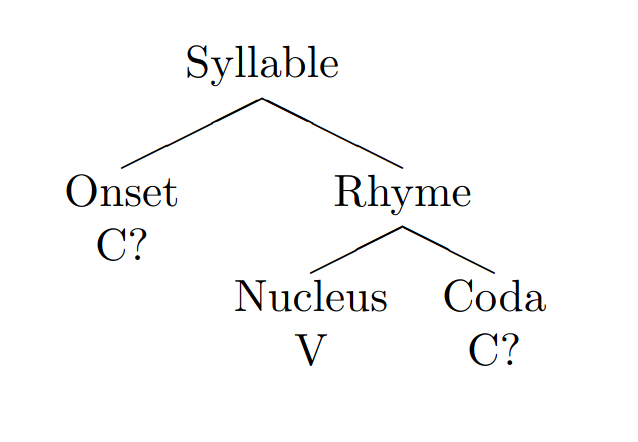
\includegraphics[width=0.6\linewidth]{syllable}
	\caption{Structure of a syllable. C-consonant, V-vowel, ?- indicates optionality}
	% \Description{Syllable structure described as a tree}
	\label{syllable}
\end{figure}


\begin{enumerate}
	\item Every independent vowel occurring at word beginning is a syllable.

	      eg: {\mal അ} {\ipa /a/} (V) in {\mal അമ്മ} {\ipa /a.mma/} (\textit{mother})
	\item Every consonant or consonant cluster with or without vowel sign at end is a syllable.

	      eg: {\mal ക} {\ipa /ka/} (CV) in {\mal കളി} {\ipa /ka.ɭi/} (\textit{game}),

	      {\mal കി} {\ipa /ki/ }(CV) in {\mal കിളി} {\ipa /ki.ɭi/} (\textit{bird}),

	      {\mal സ്ത} {\ipa /st̪a/} (CCV) in {\mal പുസ്തകം} {\ipa /pu.st̪a.kam/} (\textit{book}),

	      {\mal ഷ്ടി} {\ipa /ʂʈi/} (CCV) in {\mal ഇഷ്ടിക} {\ipa /i.ʂʈi.ka/} (\textit{brick})


	\item If there is a \textit{chillu}, \textit{anusvara} or \textit{visarga} at the end of case 1 or 2 described above, it becomes the coda and joins to the previous syllable.

	      eg: {\mal വൻ} {\ipa /ʋan/} (CVC) in {\mal അവൻ}  {\ipa /a.ʋan/ }(\textit{he}),

	      {\mal അം} {\ipa /am/} (VC) in {\mal അംബുജം} {\ipa /am.bu.ɟam/} (\textit{lotus}),

	      {\mal സ്ത്രം} {\ipa /st̪ram/} (CCCVC) in {\mal അസ്ത്രം} {\ipa /a.st̪ram/} (\textit{arrow})


	\item A consonant or consonant cluster followed by a \textit{virama} preceded by optional u-vowel ({\mal  ു}) sign, if and only if at word ends, is a syllable. In this scenario, the vowel sound is schwa {\ipa /ə/}, which does not have an explicit vowel grapheme in Malayalam.

	      eg:  {\mal ന്} {\ipa /nə/} (CV) in {\mal അവന്} {\ipa /a ʋa nə/} (\textit{him}),

	      {\mal ട്ട്} {\ipa /ʈʈə/} (CCV) in {\mal പട്ട്} {\ipa /pa ʈʈə/} (\textit{silk}),

	      {\mal ട്ടു്} {\ipa /ʈʈə/} (CCV) in {\mal പട്ടു്} {\ipa /pa ʈʈə/} (\textit{silk}),

\end{enumerate}


A sequence of characters that do not belong to any of the classes listed above, will not form a valid syllable and can not be accepted for pronunciation analysis. A vowel sign following an independent vowel ({\mal അി}), a word beginning with a virama ({\mal ്ക്കം}), an independent vowel after a consonant ({\mal കിഅ}) etc. are  examples of invalid sequences.

